\begin{figure}[h]
\centering
\begin{tikzpicture}[
node distance = 15mm and 15mm,
V/.style = {circle, fill, draw=black, inner sep=1pt, font=\footnotesize},
every edge quotes/.style = {auto, font=\footnotesize},
arrow/.style={->,semithick}
]
\begin{scope}[nodes=V]
  \node[label=above left:\( b \)] (1) {};
  \node[label=above right:\( r \)] (2) [right=of 1]  {};
  \node[label=below right:\( g \)] (3) [below=of 2]  {};
  \node[label=below left:\( o \)] (4) [below=of 1]  {};
\end{scope}
\draw[arrow]
        (1)  edge["\( br \)"] (2)
        (2)  edge["\( rg \)"] (3)
        (3)  edge["\( go \)"] (4)
        (4)  edge["\( ob \)"] (1);
\end{tikzpicture}
\caption{The HIT \( C_4 \) which is one of the types in \( \BAutoso \)}
\end{figure}

\begin{figure}[h]
\centering
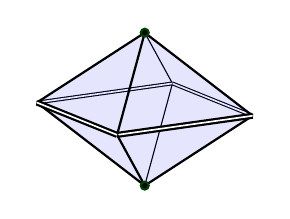
\begin{tikzpicture}%
  [x={(-0.860769cm, -0.121512cm)},
  y={(0.508996cm, -0.205391cm)},
  z={(-0.000053cm, 0.971107cm)},
  scale=1,
  back/.style={thin},
  dim2back/.style={double, thin},
  edge/.style={black, thick},
  dim2edge/.style={black, double, thick},
  facet/.style={fill=blue!95!black,fill opacity=0.1},
  vertex/.style={inner sep=1pt,circle,draw=green!25!black,fill=black,thick},
  dim1vertex/.style={}]
\coordinate (-1, -1, 0) at (-1, -1, 0);
\coordinate (-1, 1, 0) at (-1, 1, 0);
\coordinate (0, 0, -1) at (0, 0, -1);
\coordinate (0, 0, 1) at (0, 0, 1);
\coordinate (1, -1, 0) at (1, -1, 0);
\coordinate (1, 1, 0) at (1, 1, 0);
%% Drawing edges in the back
%%
\draw[edge,dim2back] (-1, -1, 0) -- (-1, 1, 0);
\draw[edge,back] (-1, -1, 0) -- (0, 0, -1);
\draw[edge,back] (-1, -1, 0) -- (0, 0, 1);
\draw[edge,dim2back] (-1, -1, 0) -- (1, -1, 0);
%% Drawing vertices in the back
%%
\node[dim1vertex] at (-1, -1, 0)     {};
%% Drawing the facets
%%
\fill[facet] (1, 1, 0) -- (0, 0, -1) -- (1, -1, 0) -- cycle {};
\fill[facet] (1, 1, 0) -- (0, 0, 1) -- (1, -1, 0) -- cycle {};
\fill[facet] (1, 1, 0) -- (-1, 1, 0) -- (0, 0, 1) -- cycle {};
\fill[facet] (1, 1, 0) -- (-1, 1, 0) -- (0, 0, -1) -- cycle {};
%% Drawing edges in the front
%%
\draw[edge] (-1, 1, 0) -- (0, 0, -1);
\draw[edge] (-1, 1, 0) -- (0, 0, 1);
\draw[dim2edge] (-1, 1, 0) -- (1, 1, 0);
\draw[edge] (0, 0, -1) -- (1, -1, 0);
\draw[edge] (0, 0, -1) -- (1, 1, 0);
\draw[edge] (0, 0, 1) -- (1, -1, 0);
\draw[edge] (0, 0, 1) -- (1, 1, 0);
\draw[dim2edge] (1, -1, 0) -- (1, 1, 0);
%% Drawing the vertices in the front
%%
\node[dim1vertex] at (-1, 1, 0)     {};
\node[vertex] at (0, 0, -1)     {};
\node[vertex] at (0, 0, 1)     {};
\node[dim1vertex] at (1, -1, 0)     {};
\node[dim1vertex] at (1, 1, 0)     {};
\end{tikzpicture}
\caption{The HIT \( \Sigma C_4 \) which has 2 points, 4 1-paths, 4 2-paths.}
\end{figure}

\begin{figure}[h]
\centering
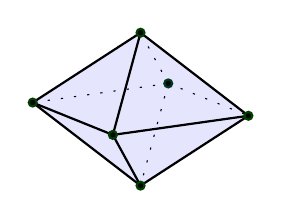
\begin{tikzpicture}%
  [x={(-0.860769cm, -0.121512cm)},
  y={(0.508996cm, -0.205391cm)},
  z={(-0.000053cm, 0.971107cm)},
  scale=1,
  back/.style={loosely dotted, thin},
  edge/.style={black, thick},
  facet/.style={fill=blue!95!black,fill opacity=0.1},
  vertex/.style={inner sep=1pt,circle,draw=green!25!black,fill=black,thick}]
\coordinate (-1, -1, 0) at (-1, -1, 0);
\coordinate (-1, 1, 0) at (-1, 1, 0);
\coordinate (0, 0, -1) at (0, 0, -1);
\coordinate (0, 0, 1) at (0, 0, 1);
\coordinate (1, -1, 0) at (1, -1, 0);
\coordinate (1, 1, 0) at (1, 1, 0);
%% Drawing edges in the back
%%
\draw[edge,back] (-1, -1, 0) -- (-1, 1, 0);
\draw[edge,back] (-1, -1, 0) -- (0, 0, -1);
\draw[edge,back] (-1, -1, 0) -- (0, 0, 1);
\draw[edge,back] (-1, -1, 0) -- (1, -1, 0);
%% Drawing vertices in the back
%%
\node[vertex] at (-1, -1, 0)     {};
%% Drawing the facets
%%
\fill[facet] (1, 1, 0) -- (0, 0, -1) -- (1, -1, 0) -- cycle {};
\fill[facet] (1, 1, 0) -- (0, 0, 1) -- (1, -1, 0) -- cycle {};
\fill[facet] (1, 1, 0) -- (-1, 1, 0) -- (0, 0, 1) -- cycle {};
\fill[facet] (1, 1, 0) -- (-1, 1, 0) -- (0, 0, -1) -- cycle {};
%% Drawing edges in the front
%%
\draw[edge] (-1, 1, 0) -- (0, 0, -1);
\draw[edge] (-1, 1, 0) -- (0, 0, 1);
\draw[edge] (-1, 1, 0) -- (1, 1, 0);
\draw[edge] (0, 0, -1) -- (1, -1, 0);
\draw[edge] (0, 0, -1) -- (1, 1, 0);
\draw[edge] (0, 0, 1) -- (1, -1, 0);
\draw[edge] (0, 0, 1) -- (1, 1, 0);
\draw[edge] (1, -1, 0) -- (1, 1, 0);
%% Drawing the vertices in the front
%%
\node[vertex] at (-1, 1, 0)     {};
\node[vertex] at (0, 0, -1)     {};
\node[vertex] at (0, 0, 1)     {};
\node[vertex] at (1, -1, 0)     {};
\node[vertex] at (1, 1, 0)     {};
\end{tikzpicture}
\caption{The HIT \( \{w, y\}* C_4 \) which has 6 points, 12 1-paths, 8 2-paths.}
\end{figure}
